\chapter{Mod\'elisation}


	En d\'eveloppement logiciel, la mod\'elisation est le fait d'associer une repr\'esentation abstraite et simplifi\'ee \`a un syst\`eme en vue de d\'ecrire sa structure, expliquer son fonctionnement, pr\'evoir des aspects de son comportement, et aussi de disposer d'un langage commun entre le client et l'\'equipe de d\'eveloppeurs.
	
	\section{UML}
		UML est un langage graphique qui permet de cr\'eer des mod\`eles qui serviront de support \`a la cr\'eation d'un syst\`eme. \\
		Le langage fournit 13 diagrammes repr\'esentant chacun une vue distincte du syst\`eme. Mod\'eliser un syst\`eme avec UML consiste \`a s\'electionner, parmi les 13 disponibles, ceux qui sont les plus adapt\'es au projet et qui, mis ensemble, le d\'ecrivent compl\`etement.\\
		
		
	\section{Diagramme de contexte}
		Le diagramme de contexte (Voir Figure~\ref{DiagrammeDeContexte}) montre relation entre un syst\`eme et les entit\'es externes qui interagissent avec lui. Notre syst\`eme interagit avec nos utilisateurs externes, \`a savoir le simple\_Utilisateur, l'administrateur et le SuperAdmin.
		
		\begin{figure}[!ht]
			\centering
			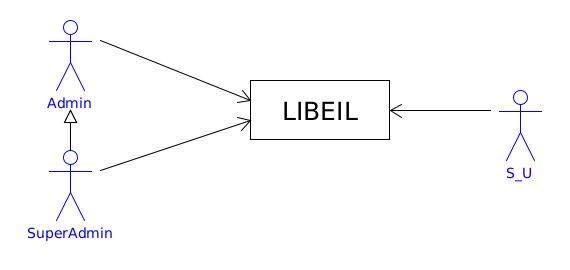
\includegraphics[width=0.5\linewidth]{Pictures/DiagrammeDeContexte.jpg}
			\caption{Le diagramme de contexte}
			\label{DiagrammeDeContexte}
		\end{figure}

	\section{Diagramme des cas d'utilisation}
		Les diagrammes de cas d'utilisation font ressortir les fonctionnalit\'es du syt\`eme que les utilisateurs vont exploiter pour interagir avec le syst\`eme.
		
		\paragraph{} Ci-apr\`es, nous pr\'esentons nos trois cas d'utilisations, \`a savoir le cas du simple\_utilisateur (Voir figure~\ref{CasUtilisationSU}), le cas de l'administrateurs (Voir figure~\ref{CasUtilisationAdmin}) et celui du SuperAdmin (Voir figure~\ref{CasUtilisationSuperAdmin}).
							
			
			
		\begin{figure}[!ht]
			\begin{minipage}{0.5\textwidth}
				\centering
				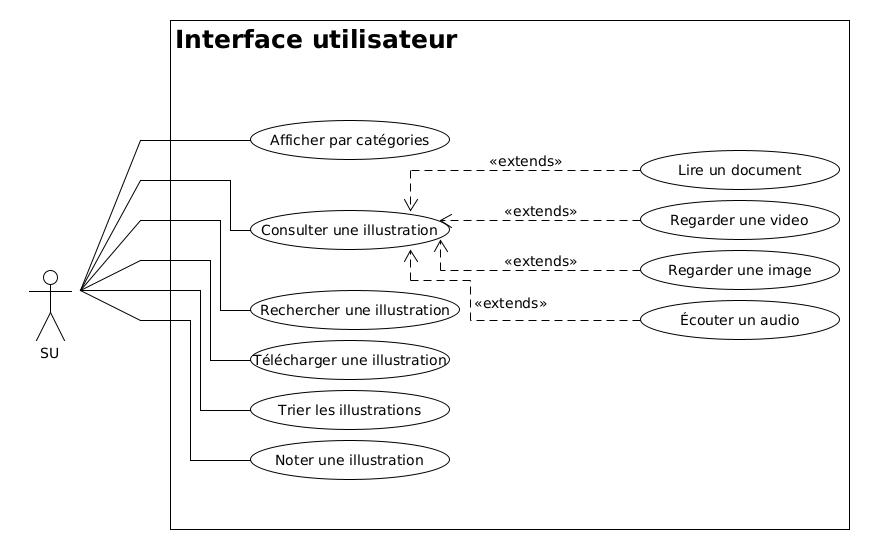
\includegraphics[width=0.9\linewidth]{Pictures/DiagrammeDesCasDUtilisationSU.jpg}
				\caption{Cas de Simple\_Utilisateur}
				\label{CasUtilisationSU}
			\end{minipage}
			\begin{minipage}{0.5\textwidth}
				\centering
				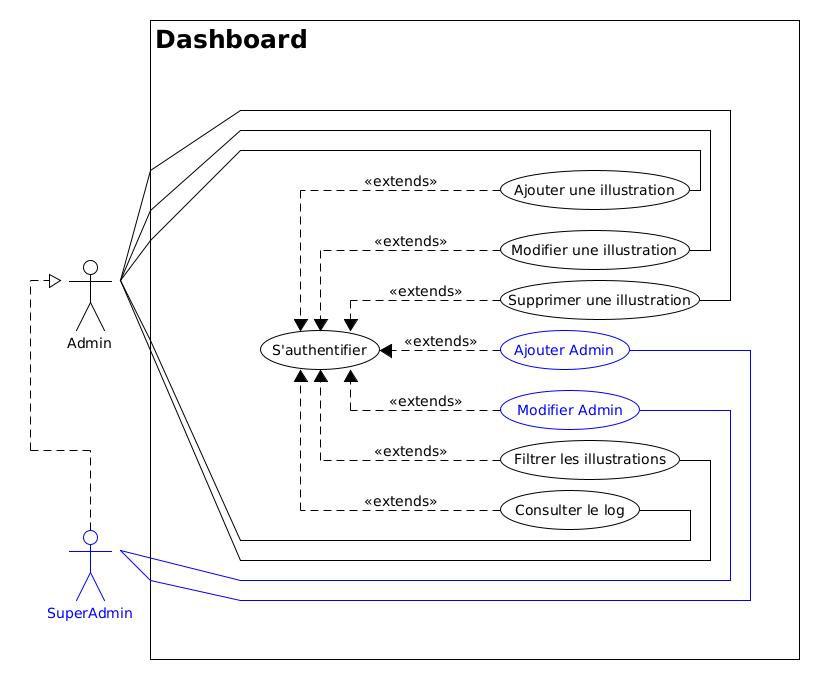
\includegraphics[width=0.9\linewidth]{Pictures/DiagrammeDesCasDUtilisationAdmin.jpg}
				\caption{Cas d'utilisation-Administrateurs}
				\label{CasUtilisationAdmin}
			\end{minipage}
		\end{figure}
			
			
	\section{Diagramme d'activit\'es}
		Le diagramme d'activit\'es (voir figure~\ref{DiagrammeDActivite}) repr\'esente le flux des activit\'es que les utilisateurs peuvent effectuer sur le syst\`eme. Il montre le flux de travail entre les utilisateurs et le syst\`eme \cite{DiagActivite}. Ce diagramme permet de mieux comprendre l'ordre dans lequel les op\'erations sont effectu\'ees et la fa\c{c}on dont elle sont coordonn\'ees. \\
			
			
			\begin{figure}[!ht]
				\centering
				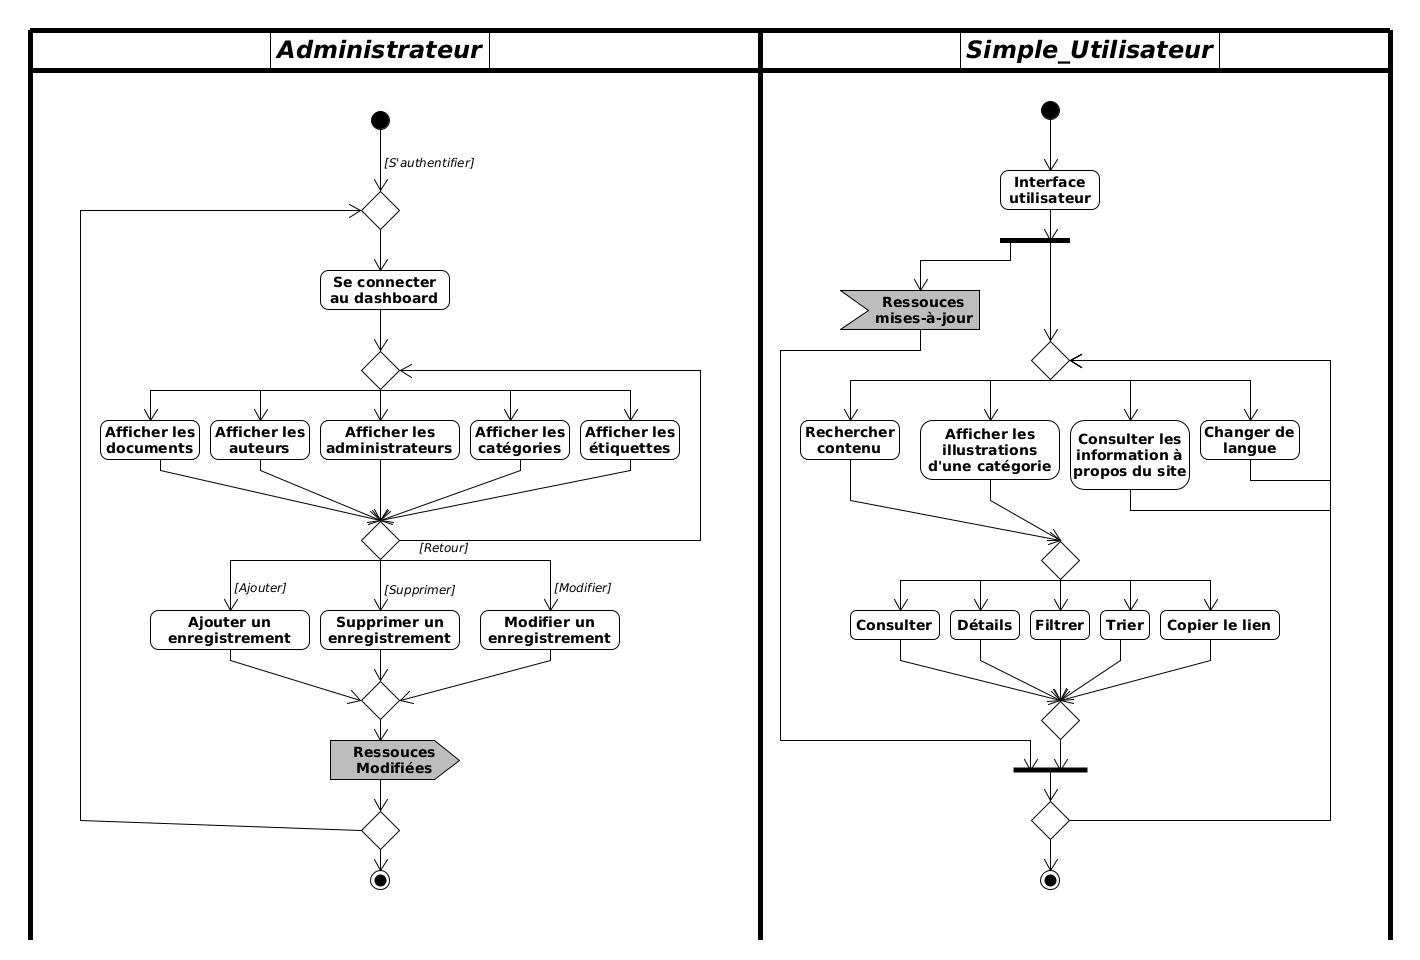
\includegraphics[width=0.75\linewidth]{Pictures/DiagrammeDActivites.jpg}
				\caption{Le diagramme d'activit\'es}
				\label{DiagrammeDActivite}
			\end{figure}
			
			
			

	\section{Diagramme de classes}

		
		Le diagramme de classe d\'ecrit la structure interne du syst\`eme en visualisant les diff\'erents types d'objets qui le constituent et les types de relations qui existent entre eux. Ce diagramme est fondamental pour la mod\'elisation du syst\`eme.
		
		\paragraph{} Dans notre cas, le diagramme des classes (voir Figure~\ref{DiagremmeClasses}) pr\'esente les 8  entit\'es du site, leur m\'ethodes ainsi que les relations entre elles.
	
		\begin{figure}[!ht]
			\centering
			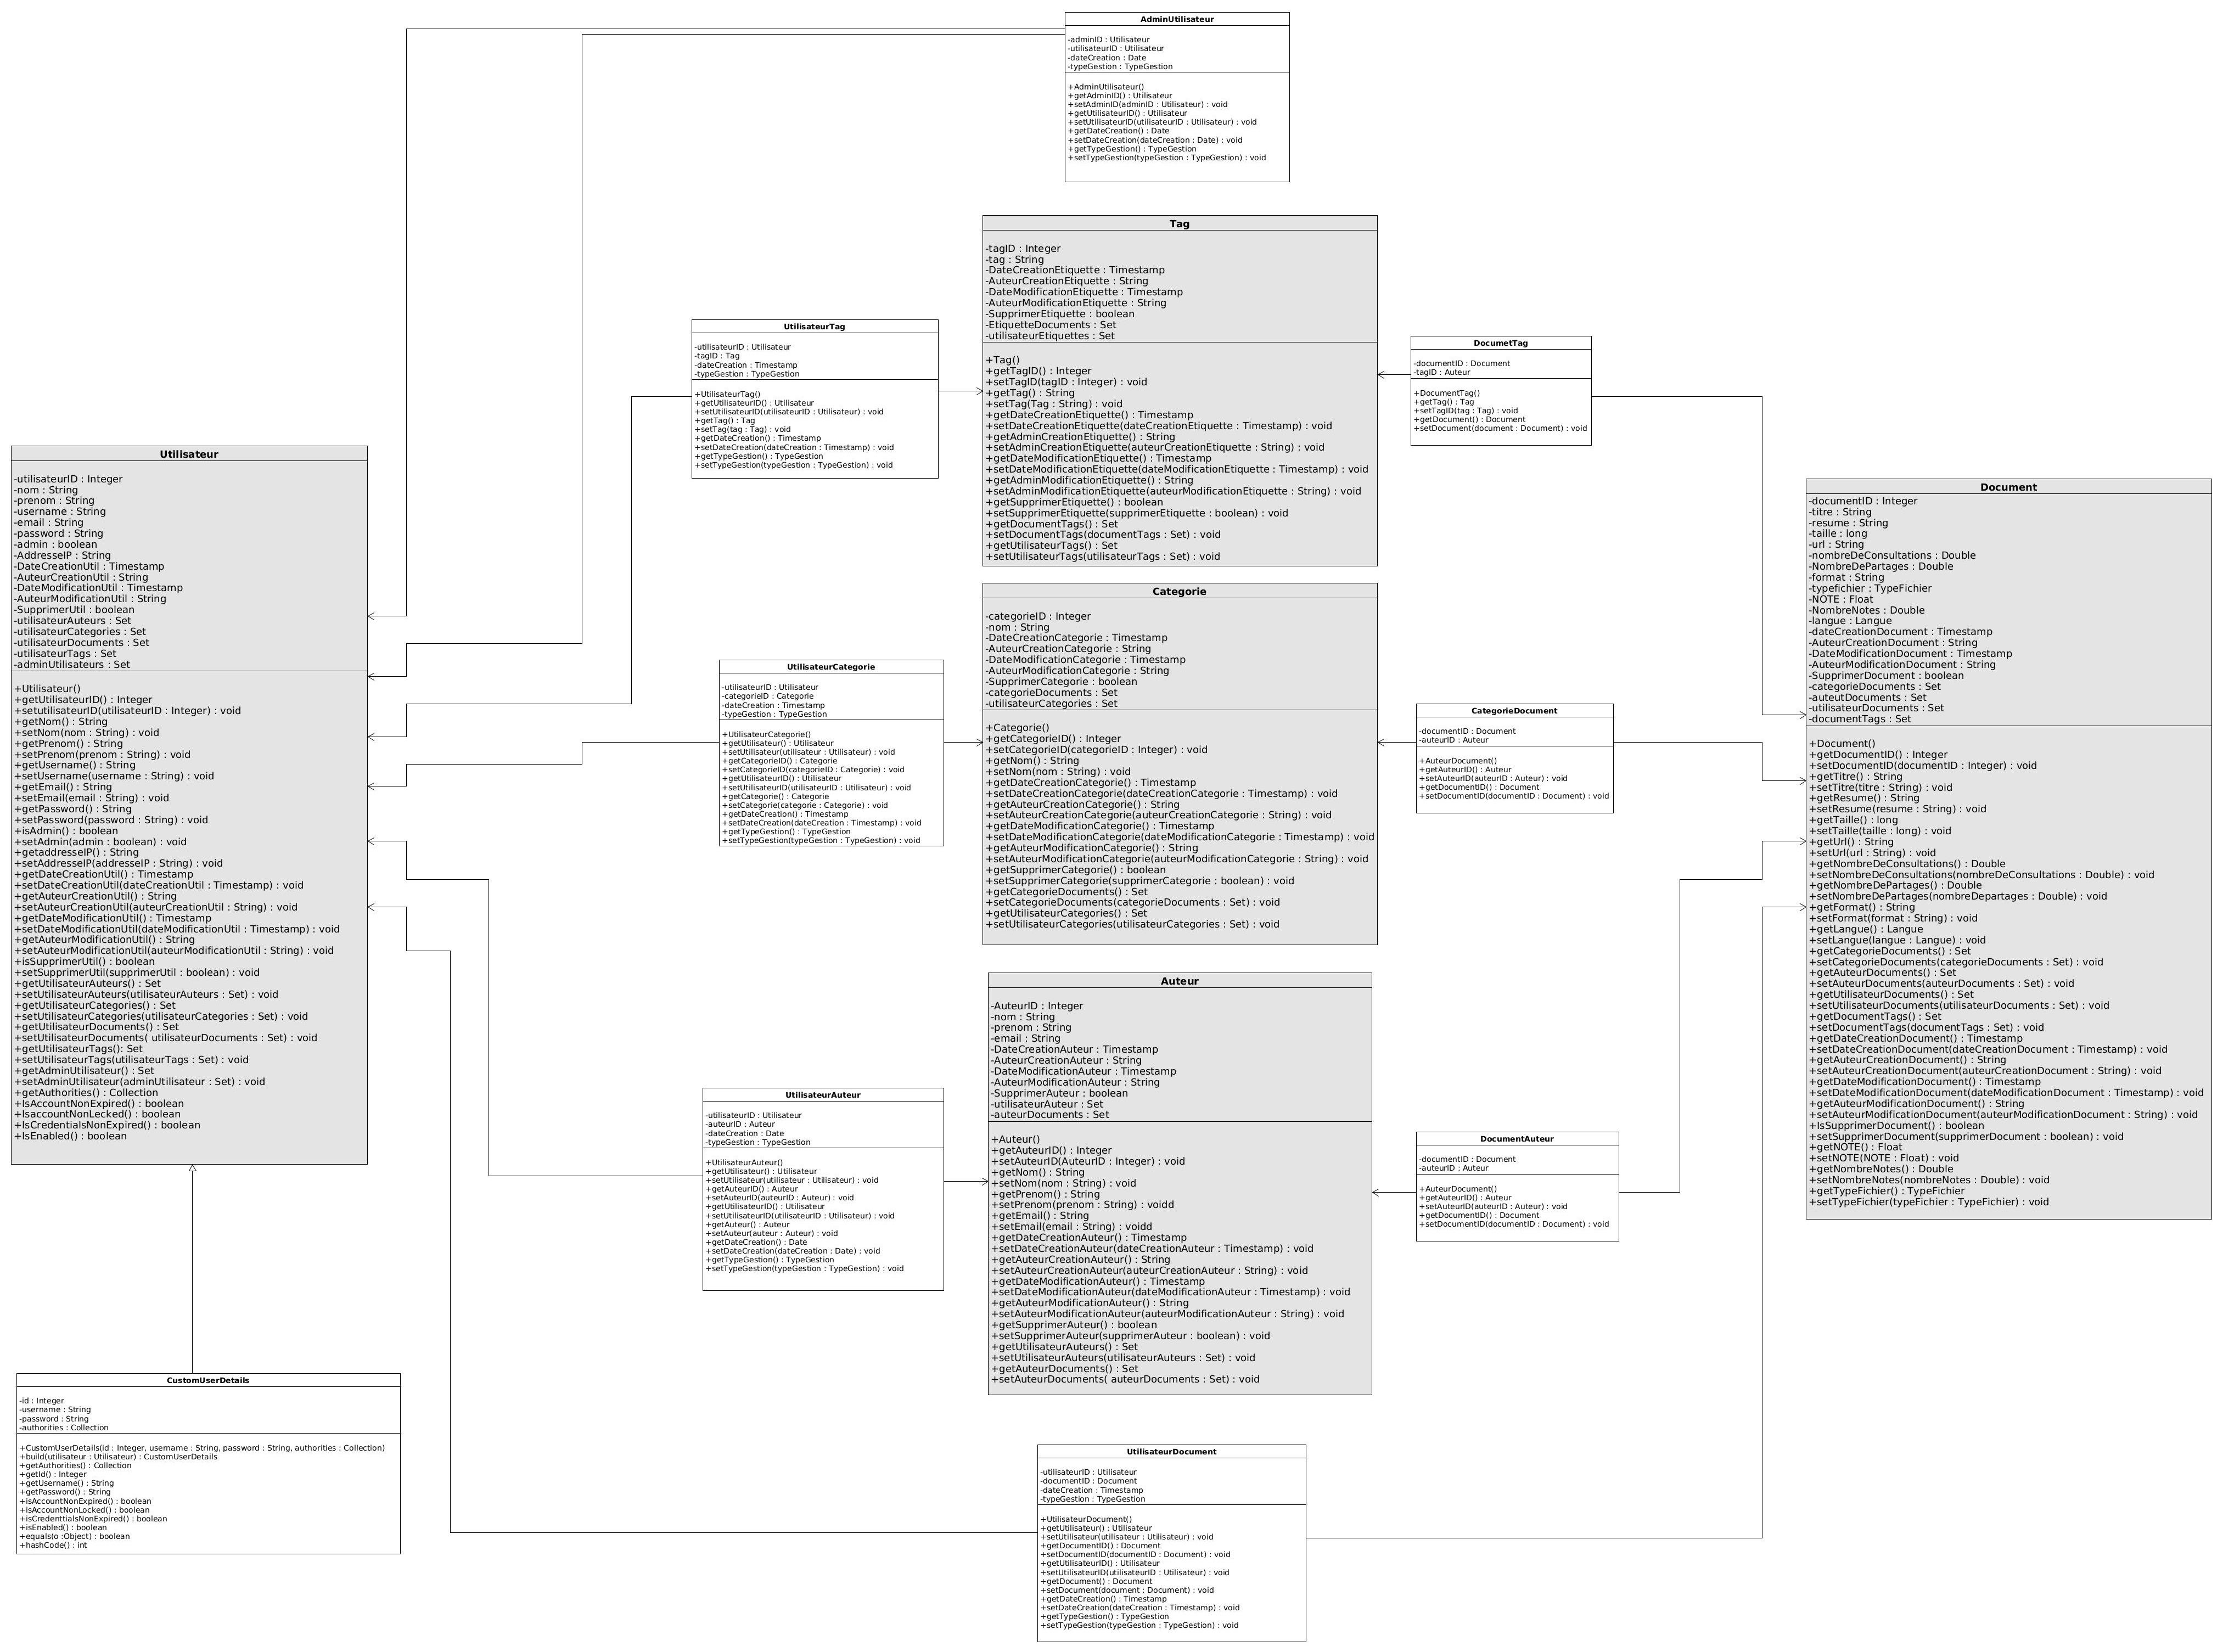
\includegraphics[width=0.7\linewidth]{Pictures/DiagrammeDeClasses.jpg}
			\caption{Le diagramme des classes}
			\label{DiagremmeClasses}
		\end{figure}



	\section{Diagrammes de s\'equence}
		Le diagramme de s\'equence repr\'esente les principaux objets qui constituent le logiciel et la suite de requ\^etes et messages entre les objets au cours des op\'erations CRUD \`a travers celui-ci. Il montre comment divers composants d'un syst\`eme interagissent les uns avec les autres pour accomplir chacune des t\^aches \cite{DiagrammeSequence}. 
		
		\subsection{Cas du simple\_utilisateur}
			\begin{figure}[!ht]
				\centering
				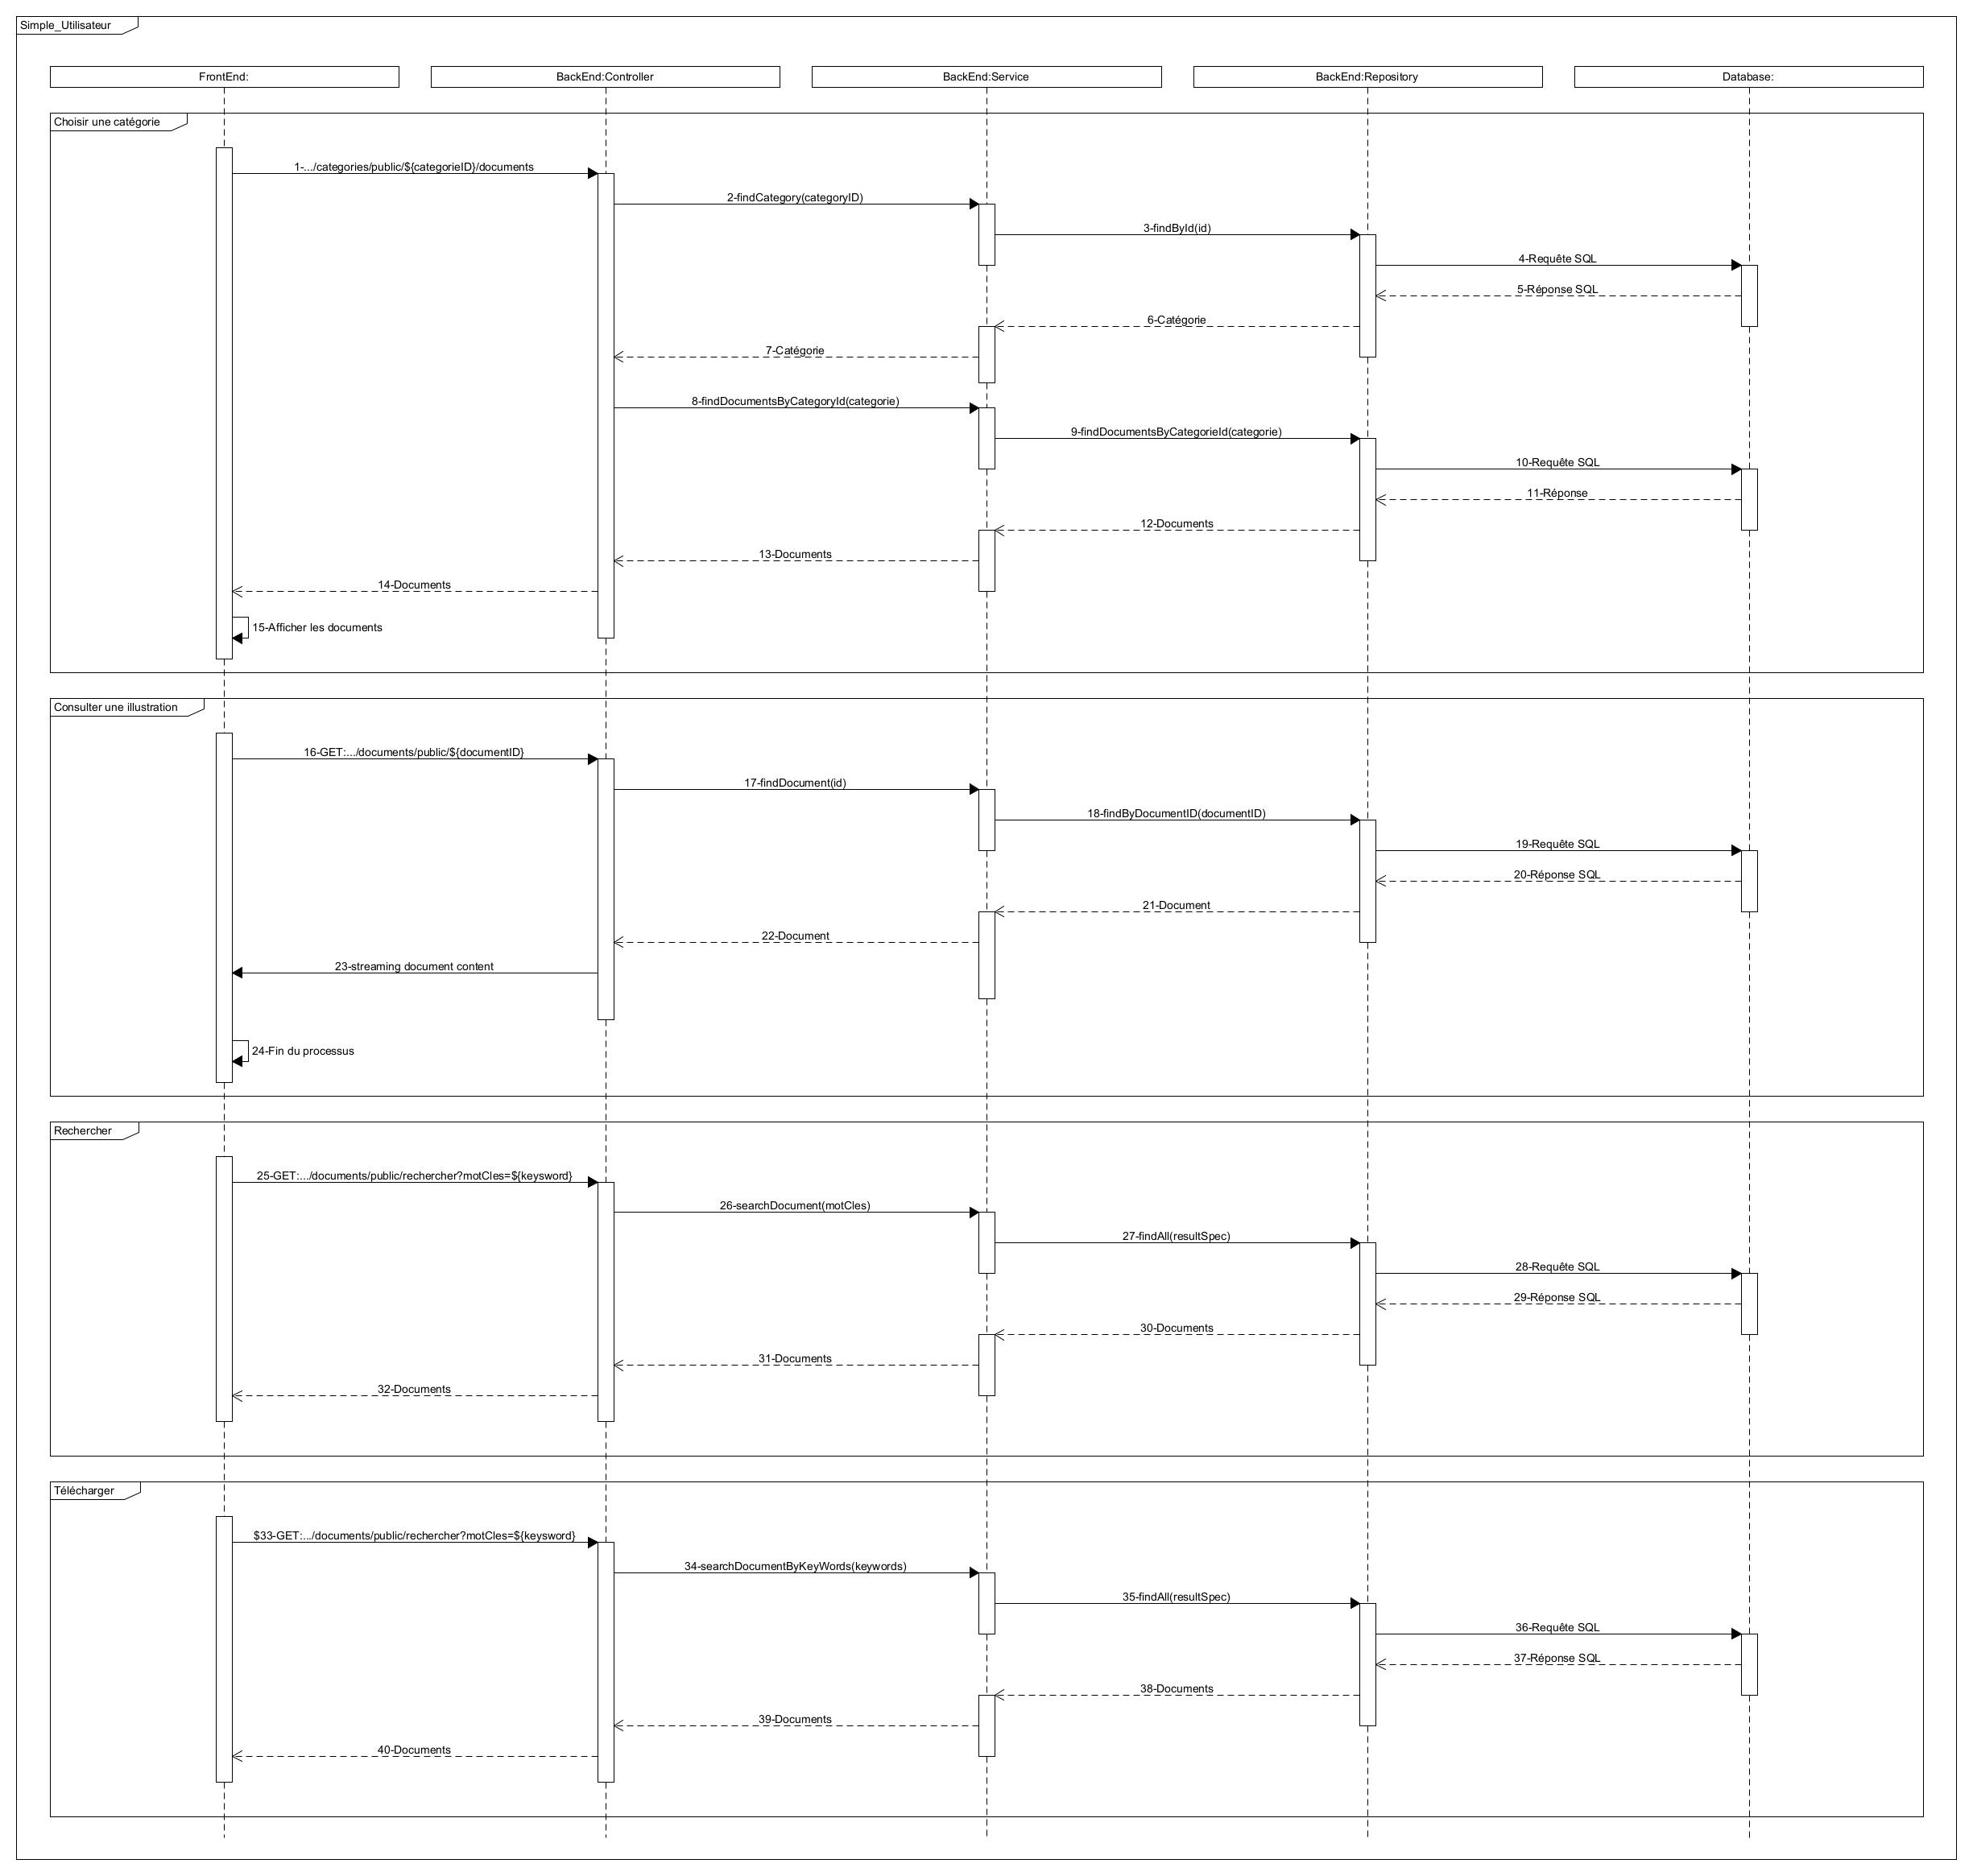
\includegraphics[height=0.7\textheight]{Pictures/DiagrammeDeSequenceSimpleUtilisateur.jpg}
				\caption{Le diagramme de s\'equences - Cas du simple\_utilisateur}
				\label{DiagrammeDeSequenceSU}
			\end{figure}

		\newpage
		\subsection{Cas de l'administrateur}
			\begin{figure}[ht]
				\centering
				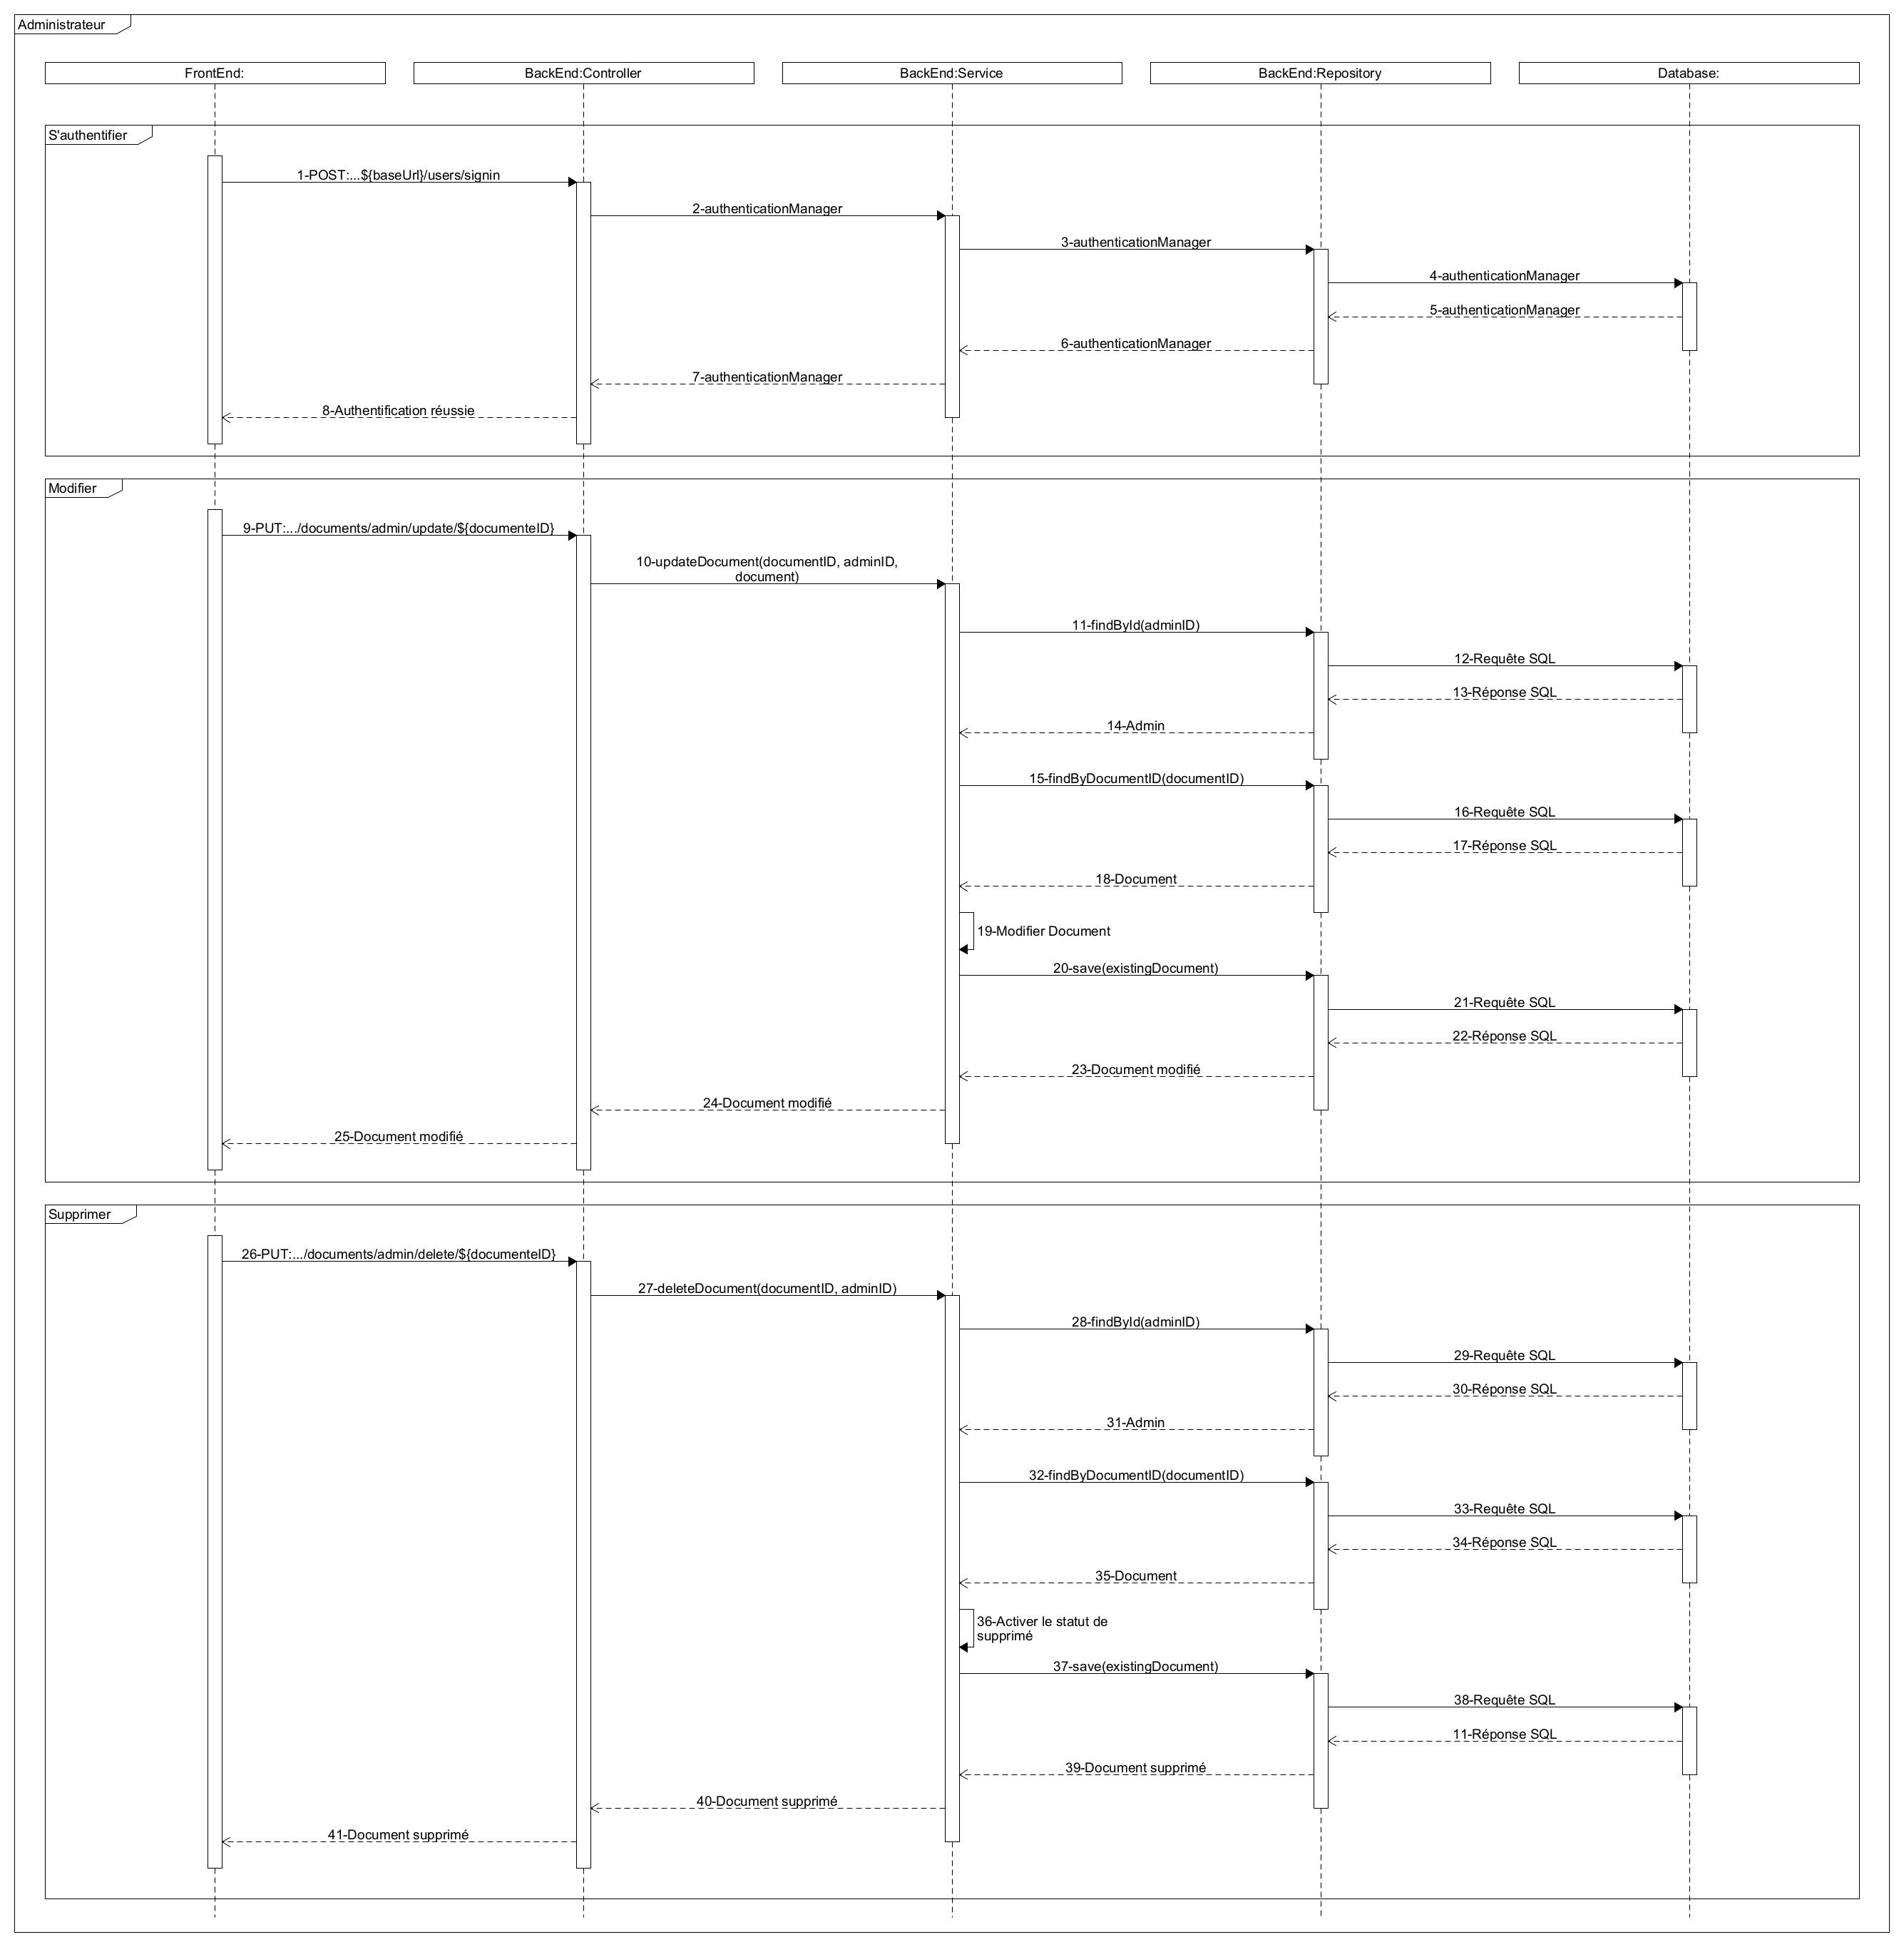
\includegraphics[height=0.7\textheight]{Pictures/DiagrammeDeSequenceAdministrateur.jpg}
				\caption{Le diagramme de s\'equences - Cas de l'administrateur-Partie 1}
				\label{DiagrammeDeSequenceAdmin1}
			\end{figure}
			
			\begin{figure}[ht]
			\centering
			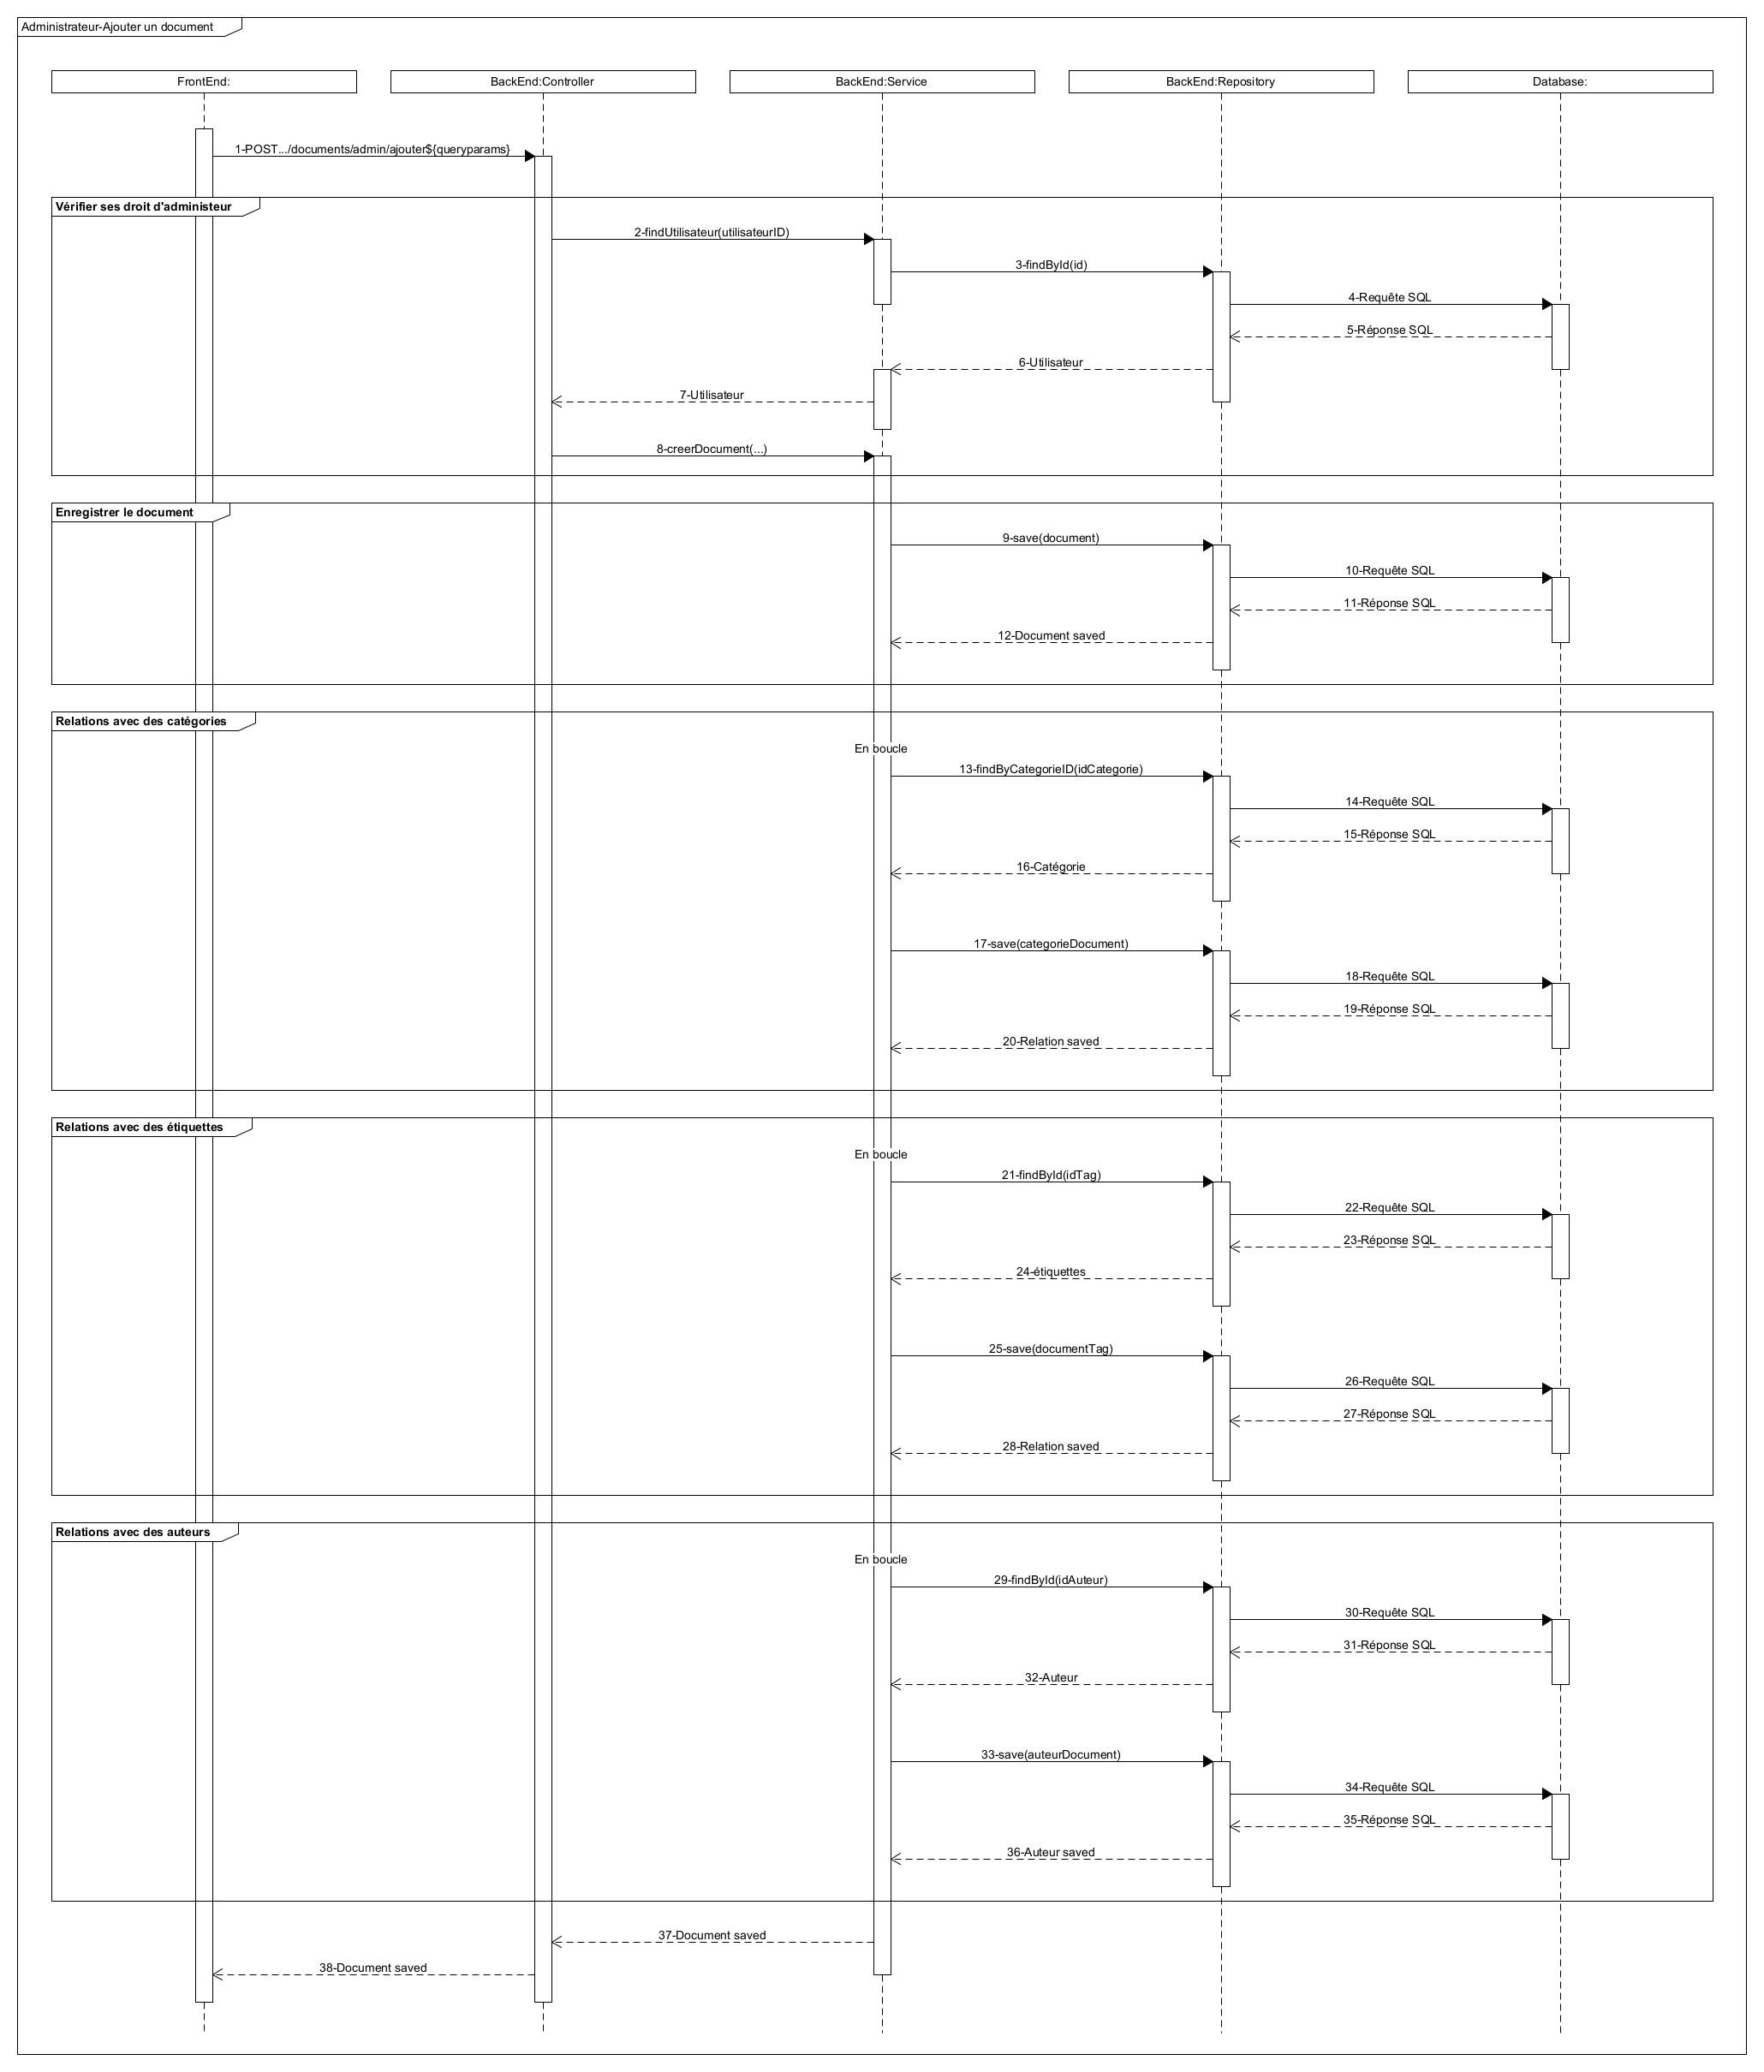
\includegraphics[height=0.7\textheight]{Pictures/DiagrammeDeSequenceAJouterDocument.jpg}
			\caption{Le diagramme de s\'equences - Cas de l'administrateur-Partie 2}
			\label{DiagrammeDeSequenceAdmin2}
			\end{figure}



